\documentclass[10pt,twocolumn]{article}

\usepackage[english]{babel}
\usepackage[utf8]{inputenc}
\usepackage{mathtools}
\usepackage{graphicx}
\usepackage[colorinlistoftodos]{todonotes}
\usepackage[margin=0.9in]{geometry}
\usepackage{multicol}

\usepackage{csquotes}
\usepackage[style=verbose-ibid,backend=biber]{biblatex}
\bibliography{sample}

\title{Using Q-Learning in Sokoban: Performance Enhancements and Challenges}

\author{
  J. Tremblay\textsuperscript{1}\thanks{\texttt{jeremy-tremblay@outlook.fr}}  
  \space et T. Guyomard\textsuperscript{1}\thanks{\texttt{thomas.guyomard@etu.univ-littoral.fr}} \\
  \textsuperscript{1}Université du Littoral Côte d'Opale, Calais, France
}

\date{\today}

\begin{document}
\maketitle

\begin{abstract}
    This paper explores the application of Q-Learning to the game Sokoban, focusing on various performance enhancements and challenges encountered. Despite its simplicity, Sokoban presents significant challenges for reinforcement learning algorithms due to its complex state space and delayed rewards. We developed several versions of a Q-Learning algorithm with modifications such as wall detection, elimination of unnecessary actions, and reward system adjustments. Experimental results demonstrate varying degrees of improvement in performance with these enhancements. However, one of the primary limitations encountered was the particularly long training times required for effective learning. Our findings provide insights into the limitations and potential of Q-Learning in Sokoban, highlighting areas for future research and application.
\end{abstract}

\section{Introduction}

Reinforcement learning (RL), a branch of machine learning, has transformed how algorithms learn to make decisions by interacting with environments to maximize cumulative rewards. Among RL techniques, Q-Learning stands out for its simplicity and effectiveness in learning optimal policies through iterative trial and error.

Adapted extensively in video games, Q-Learning excels in environments where decisions influence future states and outcomes. Sokoban, a classic puzzle game where players push boxes to designated locations, presents unique challenges for reinforcement learning algorithms due to its vast state space and delayed rewards. Each action in Sokoban can have intricate consequences, making effective strategy learning challenging without extensive training and fine-tuning.

This study explores these challenges and aims to enhance Q-Learning's effectiveness in Sokoban through modifications such as wall detection, action reduction, and adjustments to the reward system. Despite advancements, a significant limitation encountered is the extended training times necessary for effective learning. These findings contribute to understanding Q-Learning in complex environments, suggesting avenues for future research and practical applications.


\section{Related Works}

Previous studies have demonstrated the effectiveness of Q-Learning and deep reinforcement learning techniques in various gaming environments. Mnih et al. (2013) pioneered the use of deep Q-Learning to learn game policies directly from pixel inputs, achieving human-level performance on multiple classic Atari games.

In the realm of real-time strategy games, Vinyals et al. (2019) showcased advanced Q-Learning and reinforcement learning methods in achieving Grandmaster level performance in StarCraft II. Their work exemplifies the application of sophisticated learning algorithms to master complex strategic environments.

These studies highlight the versatility of Q-Learning in adapting to diverse gaming dynamics, from classic Atari games to complex real-time strategy scenarios like StarCraft II. In contrast, the challenges specific to Sokoban, such as sparse rewards and intricate state transitions, remain less explored. This study aims to address these challenges and enhance Q-Learning's applicability in puzzle-solving domains.

\section{Theoretical Foundations}

\subsection{Q-Learning Basics}

Q-Learning is a reinforcement learning technique used to learn optimal actions to take in a given state to maximize cumulative rewards. At its core, Q-Learning maintains a Q-Table (or Q-Function), denoted as \( Q(s, a) \), where \( s \) represents a state and \( a \) an action. The table is updated iteratively based on the Bellman equation:

\[
    Q(s, a) \leftarrow (1 - \alpha) \cdot Q(s, a) + \alpha \cdot \left( r + \gamma \cdot \max_{a'} Q(s', a') \right)
\]

Here, \\
- \( \alpha \) (learning rate) controls how much new information overrides old information. \\
- \( \gamma \) (discount factor) determines the importance of future rewards. \\
- \( r \) is the immediate reward received after taking action \( a \) in state \( s \). \\
- \( s' \) is the resulting state after taking action \( a \). \\

The Q-Table stores the expected future rewards for all state-action pairs, guiding the agent's decision-making process during exploration and exploitation phases.

\subsection{Exploration-Exploitation Trade-off}

In Q-Learning, \( \epsilon \) controls the exploration-exploitation trade-off, crucial for learning optimal strategies in dynamic environments. The \( \epsilon \)-greedy policy dictates action selection:

\[
    \pi(a|s) =
    \begin{cases}
        1 - \epsilon + \frac{\epsilon}{|\mathcal{A}(s)|}, & \text{if } a = \arg\max_{a'} Q(s, a') \\
        \frac{\epsilon}{|\mathcal{A}(s)|},                & \text{otherwise}
    \end{cases}
\]

Here, \( Q(s, a) \) denotes the Q-value of action \( a \) in state \( s \), \( \mathcal{A}(s) \) represents the set of possible actions in state \( s \), and \( |\mathcal{A}(s)| \) is the number of actions available in state \( s \).

Initially set high (e.g., 1.0), \( \epsilon \) encourages exploration early in training. As training progresses, \( \epsilon \) is generally reduced to prioritize exploitation of learned actions.

\subsection{Implementation Details}

In our implementation, we focused on guiding the agent's behavior through a carefully designed reward system. The system was crucial in reinforcing desired actions, such as pushing boxes onto targets, while discouraging undesired actions like pushing boxes off targets. These rewards were iteratively adjusted to improve the agent's learning process and performance in solving the Sokoban puzzle efficiently.

State representation involved converting the Sokoban map into a numerical format to ensure state uniqueness and reduce complexity. This approach facilitated effective learning and decision-making by the Q-Learning algorithm.

\section{Methodology}

\subsection{Tools}

The implementation was conducted using Python programming language, leveraging the Gym Sokoban library. Gym Sokoban provides a simulated environment for the Sokoban game, facilitating the integration of reinforcement learning algorithms for experimentation and evaluation.

\subsection{Initialization of Q-Learning}

To evaluate the effectiveness of Q-Learning in the Sokoban game context, we began by implementing a basic Q-Learning algorithm using the Gym Sokoban library in Python. The Q-Table was initialized with default parameters ($\alpha$ = 0.5, $\gamma$ = 0.95, $\epsilon$ = 0.1).

\subsection{Reward System}

The initial reward system was defined as follows:
\begin{itemize}
    \item Performing an action: -0.1
    \item Pushing a box onto a target: +1.0
    \item Pushing a box off target: -1.0
    \item All boxes on targets: +10.0
\end{itemize}

\subsection{State Representation}

To ensure state uniqueness, we converted the Sokoban map into a numerical representation and hashed it to obtain a unique state identifier. This approach reduced state complexity while preserving uniqueness.

\subsection{Iterative Improvements}

We introduced several modifications to enhance Q-Learning performance:
\begin{itemize}
    \item Detection of losing conditions to avoid ineffective actions.
    \item Restriction of the "do nothing" action to promote active movements.
    \item Optimization of alpha, gamma, and epsilon parameters, as well as the reward system, to improve learning.
\end{itemize}

\subsection{Generalization Evaluation}

We evaluated the model's ability to generalize to new Sokoban levels by testing its performance without complete retraining. This methodology enabled us to explore the capabilities and limitations of Q-Learning in a complex gaming environment.

\section{Implementation and Results}

\subsection{Initial Q-Learning Implementation}

We began by implementing Q-Learning on a Sokoban puzzle with three boxes using the Gym Sokoban library in Python. The chosen level (Figure \ref{fig:sokoban_level}) is a representative example of Sokoban's complexity, where the agent must strategically move 3 boxes to designated target locations.

\begin{figure}[ht]
    \centering
    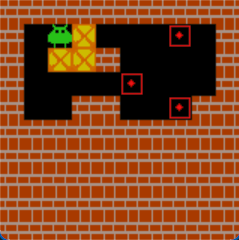
\includegraphics[width=0.3\textwidth]{Images/sokoban.png}
    \caption{Example Sokoban level used for these Q-Learning experiments.}
    \label{fig:sokoban_level}
\end{figure}

Initially, the Q-Learning agent struggled to solve the puzzle, requiring approximately 1800 episodes to achieve its first successful completion. After this initial breakthrough, the agent demonstrated improved learning efficiency, achieving successful completions in subsequent attempts approximately 60\% of the time.



\section{Conclusions}
\label{sec:conclusions}

\printbibliography

\end{document}